Many convex optimization methods can be interpreted as the discretization of an ordinary differential equation whose solution trajectories approximate the steps of the optimization algorithm. The established theory of ordinary differential equations and dynamical systems can often provide insight in the design and analysis of their corresponding discrete-time optimization algorithms. Connections between these fields have been fruitfully explored in the classical optimization literature in a number of works \citep{helmke2012optimization, schropp2000dynamical, fiori2005quasi, durr2012class, dorr2012smooth, osher2016sparse, qin2012structured, lessard2016analysis}.

In the present work we both review and advance the connection between first-order gradient methods for optimization and their continuous-time counterparts -- in particular focusing on the continuous-time limit of Nesterov's accelerated gradient method. First-order methods have regained popularity in machine learning and many other fields as data sets and problems increase in size and complexity. Thirty years ago, in a seminal paper, Nesterov proposed a family of ``accelerated" gradient algorithms provably improving upon the convergence rate of ordinary gradient descent \citep{nesterov1983method}\footnote{Nesterov proposed two distinct schemes for both accelerating gradient descent applying to both weakly and strongly convex functions -- we henceforth refer to Nesterov (I) for the scheme for weakly convex functions and Nesterov (II) for the scheme for strongly convex functions}. While these accelerated methods are easy to implement, the convergence proofs of these accelerated first-order gradient schemes have long been considered difficult to understand. Further, many researchers have also lacked an intuitive understanding of ``why" these methods work -- making them difficult to generalize as well.

A recent line of research initiated by \citet{su2014differential} derived, perhaps surprisingly, a \textit{second-order} ODE which is the exact limit of the \textit{first-order} Nesterov (I) scheme. Various examples and case studies related to this second-order ODE provided in \citet{su2014differential} used this conceptually simpler ODE as a tool for understanding, analyzing and generalizing Nesterov’s scheme. Since then, several researchers have attempted to both extend this work into more general settings and further understand the significance of the discretization between the continuous-time ODE perspective and the original discrete-time Nesterov schemes \citep{krichene2015accelerated, wibisono2016variational, wilson2016lyapunov}.

The purpose, structure, and contributions of this project can be broadly summarized as:
\begin{itemize}
    \item Reviewing accelerated first-order methods in both discrete and continuous time focusing on establishing the optimality lower bounds shown in \citet{nesterov2004introductory} and introducing the continuous-time limit analyzed in \citet{su2014differential} for the Nesterov (I) scheme.
    \item Extending results of \citet{su2014differential} to the case of the Nesterov (II) scheme which is applicable to strongly convex functions. This includes producing both continuous-time convergence proofs of exponential convergence rates for gradient descent and the Nesterov (II) scheme we derive, and providing an intuitive perspective connecting the Nesterov (II) scheme to the physics of the damped harmonic oscillator.
    \item Investigating the generalization of the Nesterov (I) scheme to non-Euclidean geometries -- i.e. ``accelerated" mirror descent -- in both discrete and continuous time as studied in \citet{krichene2015accelerated}.
\end{itemize}

\subsection{Gradient Descent}

Gradient descent is an iterative optimization algorithm that can be used to minimize a function $f$ over $\mathbb{R}^{d}$. The iterates evolve as:
\begin{equation}
    x_{k+1} = x_k - s \nabla f(x_k)
\end{equation}
where $s > 0$ is the step size. 

One can provably show the convergence of gradient descent algorithm when it is used to minimize a \textit{convex} function subject to smoothness conditions on the function $f$. In particular, depending on the type of convex function we can derive different rates of convergence for its quickness in finding the global optima of $f(x)$, $x^*$. 

\begin{figure}[!h]
\begin{center}
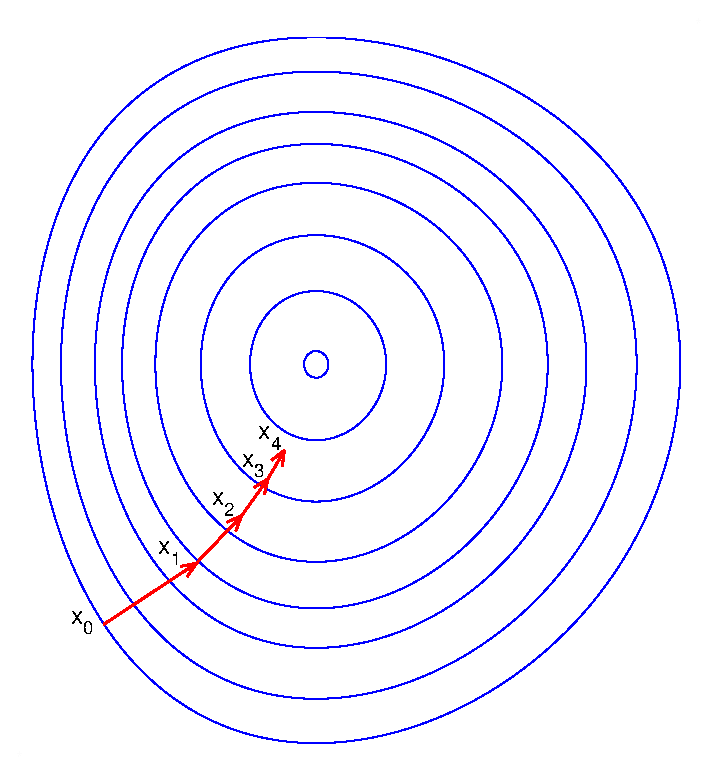
\includegraphics[width=0.2\linewidth]{SourceFiles/plots/Gradient_descent.eps}
\caption{Gradient Descent iterates moving towards the global optimum.}
\end{center}
\end{figure}

To this end, it is interesting to consider the class of functions which are restricted to being $\beta-$smooth and $\alpha-$strongly convex. 
We now recall these definitions:
\begin{definition}
If $f$ is a differentiable, convex function and $x,y$ two points in its domain, then:
\begin{equation}\label{convexity_def_eq}
f(y) \geq f(x) + \nabla f(x)^\top (y-x)
\end{equation}
\end{definition}

\begin{definition}
$f$ is $\alpha-$strongly convex if:
\begin{equation}
f(y) \geq f(x) + \nabla f(x)^\top(y-x) + \frac{\alpha}{2} ||x - y||_2^2
\end{equation}
\end{definition}

Alternatively, a function $f$ is strongly convex if $x \rightarrow f(x) - \frac{\alpha}{2} ||x||^2$ is convex. In the case of twice differentiable functions this is equivalent to $\nabla^{2} f(x) \succeq \alpha I$. Intuitively, this is equivalent to stating that $f$ is globally \textit{lower-bounded} by a quadratic function. 

\begin{definition}
$f$ is $\beta$-smooth if:
\begin{equation}\label{fundamental_beta_eq}
f(y) \leq f(x) + \nabla f(x)^\top(y-x)+ \frac{\beta}{2} ||x - y||_2^2
\end{equation}
\end{definition}
Alternatively, a function $f(x)$ is $\beta$-smooth if its gradients $\nabla f(x)$ are $\beta-$Lipschitz:
\begin{equation}
    || \nabla f(x) - \nabla f(y) || \leq \beta ||x - y||
\end{equation}
In the case of twice differentiable functions this is equivalent to $\nabla^{2} f(x) \preceq \beta I$.
Intuitively, this is equivalent to stating that $f$ is globally \textit{upper-bounded} by a quadratic function.
\newline
If $f$ is $\alpha-$strongly convex and $\beta-$smooth then:
\begin{definition}
The \textbf{condition number} of $f$ is $\kappa = \frac{\beta}{\alpha}$. 
\end{definition}

\subsection{Convergence Rates}

It is well-known that gradient descent applied to a $\beta-$smooth functions achieves a $\mathcal{O}(1/k)$ convergence rate \citep{DBLP:journals/ftml/Bubeck15}:

\begin{theorem}
Let $f$ be convex and $\beta$-smooth, then gradient descent with $s = \frac{1}{\beta}$ satisfies:
\begin{equation}
f(x_k) - f(x^*) \leq \frac{2\beta ||x_1 - x^* ||_2^2}{k-1}
\end{equation}
\end{theorem}

If the function $f$ is smooth and strongly convex the convergence rate of gradient descent is improved from $\mathcal{O}(1/k)$ to $\mathcal{O}(\exp(-k/\kappa))$ \citep{DBLP:journals/ftml/Bubeck15}:

\begin{theorem}
If $f$ is $\alpha-$strongly convex and and $\beta-$smooth then gradient descent with step size $s = \frac{2}{\alpha+\beta}$ satisfies:
\begin{equation}
f (x_{k+1}) - f(x^*) \leq \frac{\beta}{2} \exp(-\frac{4k}{\kappa+1}) ||x_1-x^*||_2^2
\end{equation}
\end{theorem}

\begin{center}
 \begin{tabular}{||c c ||} 
 \hline
 Function Class  & Gradient Descent Convergence Rate \\ [0.5ex] 
 \hline\hline
 $\beta$-Smooth  & $\frac{1 }{k}$  \\ [1ex]
 \hline
 $\beta$-Smooth and $\alpha-$Strongly Convex   & $\exp\left(-\frac{k}{\kappa}\right)$  \\[1ex]
 \hline
\end{tabular}
\end{center}
As we will see in the next section these rates are not optimal.  \citet{blair1985problem} proved optimality lower bounds for the convergence rate of an first-order algorithm that can only access function and gradient evaluations. Remarkably, \citet{nesterov2004introductory} also presented an ``acceleration" scheme to achieve these lower bounds.

\subsection{``Oracle" Lower Bounds}

A black box optimization procedure is a mapping from the history of the algorithm to the next query point, in the algorithm's quest for the minimizer of $f$. A black-box first-order optimization algorithm is any method that produces iterates $x_{k+1}$ from the values $(x_1, g_1, \cdots, x_k, g_k)$ where $g_k \in \partial f(x_k)$. Here we restrict to ``linear", black-box procedures such that
\begin{equation}
x_{k+1} \in \text{span}(g_1, \cdots, g_k)
\end{equation}
and also assume that $x_1 = 0$ in order to simplify the notation in the proofs\footnote{Note that this is not a restriction since these proofs proceed by constructing an ``adversarial" quadratic form which the black-box procedure cannot descend arbitrarily fast. Equivalently, we could assume $x_1 \neq 0$ by simply translating these quadratic forms accordingly.}.
\citet{blair1985problem} was the first to prove lower bounds showing that any black-box, linear first-order optimization algorithm could not descend a $\beta$-smooth convex function faster than at a  $\mathcal{O}(1/k^2)$ rate and a $\alpha$-strongly convex, $\beta$-smooth function faster than at a  $\mathcal{O}(\exp(-k/\sqrt{\kappa})$ rate.

In this section, we present proofs of these lower bounds for both classes of convex functions.
Throughout this section we will use $e_1, \cdots, e_n$ to denote the canonical basis of $\mathbb{R}^n$. We first show that for $\beta$-smooth convex functions there is no linear, first-order, black-box procedure achieving a faster convergence rate than $\mathcal{O}(\frac{1}{k^2})$. 

\begin{theorem}
Let $k \leq \frac{n-1}{2}$ and $\beta>0$. Then there is a $\beta$-smooth convex function such that any black box procedure for which $x_{k+1} \in \text{span}(g_1, \cdots, g_k)$ satisfies: 
\begin{equation}
\min_{1 \leq a \leq k } f(x_a ) - f(x^*) \geq \frac{3\beta}{32} \frac{||x_1 - x^*||^2}{(k+1)^2} 
\end{equation}
\label{thm:convex1proof}
\end{theorem}

\proofstart
Consider the following quadratic form:

\begin{equation}
    f(x) = \frac{\beta}{8}x^T A_{2k+1}x- \frac{\beta}{4}x^Te_1
\end{equation}

Where $A_m$ is an $n\times n$ matrix defined as:

\begin{equation}
(A_m)_{i,j} = \begin{cases}
                2  &  i = i,j \leq k \\
                -1 &  j \in \{i-1, i+1\}, i \leq k, j \neq m+1\\
                0 & \text{else}
            \end{cases}
\end{equation}
 We can now verify the following useful properties of $A_m$, $f(x)$ and the iterates $x_m$ are satisfied:
\begin{enumerate}
\item $0 \preceq A_m \preceq 4I_n$ since $x^\top A_m x = x(1)^2 + x(m)^2 + \sum_{i=1}^{m-1} (x(i)-x(i+1))^2$.
\item If $y(i) = 0$ for $i \geq r$, then $y^\top A_{2k+1} y = y^\top A_{r}y$ and thus $\nabla f(y) \in \text{span}(e_1, \cdots, e_{r})$.  
\item $x_m$ is in the span of $(e_1, \cdots, e_{m-1})$. This follows since, without loss of generality we have assumed $x_1 = 0$ and thus $\partial f(x_1) = -\frac{\beta}{4}e_1 \implies x_2 \in \text{span}(e_1)$. An inductive application of property 2 then shows that $x_m \in \text{span}(e_1, \cdots, e_{m-1})$.
\end{enumerate}

It is now convenient to define the functions $f_m(x) = \frac{\beta}{8} x^T A_m x - \frac{\beta}{4}x^Te_1$. Simply combining all of our previous observations allows us to obtain the following series of inequalities:
\begin{equation}
f(x_m) - f^* = f_s(x_m) - f_{2k+1}^* \geq f_m^* - f^*_{2k+1} \geq f_k^* - f_{2k+1}^*
\end{equation}

Thus it simply remains to compute the minimizer $x_k^*$ of $f_k$, its norm, and the corresponding function value $f_k^*$. Note that the point $x_k^*$ is the unique solution in the span of $e_1, ..., e_k$ satisfying $A_k x = e_1$. It is then easy to verify the minimizer $x_m^*$ of $f_m(x)$ and its optimal value $f_m^*$ satisfy:
    \begin{align}
        & x_m^*(i) = \begin{cases}
                    1-\frac{i}{m+1} & i = 1, \cdots, k \\
                    0 & \text{o.w.}
                    \end{cases}\\
        & f_m^* = \frac{\beta}{8}(x^*_k)^\top A_k x_k^* - \frac{\beta}{4}(x^*_k)^\top e_1 = -\frac{\beta}{8}(x_k^*)^\top e_1 = -\frac{\beta}{8}\left( 1-\frac{1}{m+1}\right)
    \end{align}
and further that $||x_m^*||^2 = \sum_{i=1}^{m}(1-\frac{i}{k+1})^2 = \sum_{i=1}^m \left( \frac{i}{m+1}\right)^2 \leq \frac{m+1}{3}$. Thus we obtain:
\begin{equation}
f_k^* - f_{2k+1}^* =\frac{\beta}{8}\left( \frac{1}{k+1} - \frac{1}{2k+2}\right) \geq \frac{3\beta}{32} \frac{||x_{2k+1}^*||^2}{(k+1)^2} = \frac{3\beta}{32} \frac{||x_1 - x^*||^2}{(k+1)^2}
\end{equation}
concluding the proof.
\proofend


We next show that for $\alpha$-strongly convex, $\beta-$smooth functions there is no linear, first-order, black-box procedure achieving a faster convergence rate than $\mathcal{O}(\exp(-\frac{k}{\sqrt{\kappa}})$. To simplify the proof of the next theorem we will work in the limit that $n \to +\infty$: that is we are working the Hilbert space $\ell_2 = \{ x = (x(n))_{n \in \mathbb{N}} : \sum_{i=1}^{+\infty} x(i)^2 < + \infty \}$ rather than $\mathbb{R}^n$. As noted in \citet{DBLP:journals/ftml/Bubeck15} all the complexity lower bounds shown in \citet{nesterov2004introductory} are valid in arbitrary Hilbert spaces.


\begin{theorem}
Let the condition number $\kappa > 1$. Then there is a $\beta-$smooth and $\alpha-$strongly convex function $f: \ell_2 \rightarrow \mathbb{R}$ with $\kappa = \frac{\beta}{\alpha}$ such that for any $k \geq 1$ and any black box procedure for which $x_{m+1} \in \text{span}(g_1, \cdots, g_m)$:

\begin{equation}
f(x_k) - f(x^*) \geq \frac{\alpha}{2} \left(\frac{ \sqrt{\kappa}-1}{\sqrt{\kappa}+1}\right)^{2(k-1)} ||x_1 - x^*||^2
\end{equation}

When $\kappa$ is large, $\left(\frac{ \sqrt{\kappa}-1}{\sqrt{\kappa}+1}\right)^{2(k-1)} \approx \exp( -\frac{4(k-1)}{\sqrt{\kappa}})$.
\end{theorem}

\proofstart

The core ideas of this argument are quite similar to those used in Theorem \ref{thm:convex1proof}. Let $A$ the infinite-dimensional linear operator corresponding to an infinite matrix with $2$ on the diagonal, and $-1$ on the upper and lower diagonals (which generalizes the finite-dimensional $A_m$ used in the proof of Theorem \ref{thm:convex1proof}). 

We now consider the following $\alpha$-strongly convex and $\beta$-smooth function:
\begin{align*}
f(x) = \frac{\alpha(\kappa-1)}{8} \left( \langle Ax, x \rangle - 2\langle e_1, x \rangle \right) + \frac{\alpha}{2}||x||^2
\end{align*}
As before we have that $A$ satisfies $0 \preceq A \preceq 4I$ which immediately implies that $f$ is in fact $\alpha$-strongly convex and $\beta$-smooth.

Now, since $f$ is $\alpha-$strongly convex we have that $f(x_m) - f(x^*) \geq \frac{\alpha}{2} || x_m - x^* ||^2$. Thus to conclude the result we would like lower bound $||x_m - x^*||^2$. As before the crucial observation is that for this function, due to the assumptions on our black-box procedure, we have that $x_{k}(i) = 0, \forall i \geq k$. This property immediately gives that:
\begin{align*}
||x_k - x^*||^2 \geq \sum_{i=k}^\infty x^*(i)^2
\end{align*}

Now, we need only compute $x^*$. This can be done by  differentiating $f$ and setting its gradient to zero which will be achieved by the $x^*$ satisfying the following set of infinite equations:
\begin{align*}
    1-2\frac{\kappa+1}{\kappa-1} x^*(1) + x^*(2) &= 0, \\
    x^*(k-1) - 2\frac{\kappa+1}{\kappa-1} + x^*(k+1) &= 0, \qquad \forall k \geq 2
\end{align*}
which implies
\begin{align*}
x^*(i) = \left( \frac{\sqrt{\kappa} - 1}{\sqrt{\kappa} +1} \right)^i 
\end{align*}
Recalling that $x_1 =0$ and assembling these bounds shows that:
\begin{align*}
 f(x_k) - f(x^*) &\geq \frac{\alpha}{2}\sum_{i=k}^\infty \left( \frac{\sqrt{\kappa} - 1}{\sqrt{\kappa} +1} \right)^{2i}  \\
 &\geq \frac{\alpha}{2} \left( \frac{\sqrt{\kappa} - 1}{\sqrt{\kappa} +1} \right)^{2(k-1)} \left( \sum_{i=1}^\infty \left( \frac{\sqrt{\kappa} - 1}{\sqrt{\kappa} +1} \right)^{2i} \right) \\
 &\geq \frac{\alpha}{2} \left( \frac{\sqrt{\kappa} - 1}{\sqrt{\kappa} +1} \right)^{2(k-1)} || x^* ||^2 \\
 &\geq \frac{\alpha}{2} \left( \frac{\sqrt{\kappa} - 1}{\sqrt{\kappa} +1} \right)^{2(k-1)} || x_1 - x^* ||^2\\
\end{align*}
concluding the proof.

\proofend

The following table sumarizes the lower bounds above and the gradient descent rates. 

\begin{center}
 \begin{tabular}{||c c c ||} 
 \hline
 Function Class   & GD  & Lower bound \\ [0.5ex] 
 \hline\hline
 $\beta$-Smooth & $\frac{1}{k}$ &  $\frac{1}{k^2}$\\ [1ex]
 \hline
 $\beta$-Smooth, $\alpha-$Strongly Convex  &  $\exp\left(-\frac{k}{\kappa}\right)$ &  $\exp\left(-\frac{k}{\sqrt{\kappa}}  \right)$ \\ [1ex]
 \hline
\end{tabular}
\end{center}

\subsection{Accelerated Gradient Descent }

Remarkably, \citet{nesterov1983method, nesterov2004introductory} produced a family of first order methods to achieve the optimal ``oracle" lower bounds, for both weakly convex and strongly convex smooth functions, proven in \citet{blair1985problem}. We state versions of these algorithms here \citep{DBLP:journals/ftml/Bubeck15}.

For the case of $\beta$-smooth, weakly convex functions we first define the updates:

\begin{align}
\begin{split}
    x_{k+1} &= y_{k} - \frac{1}{\beta} \nabla f(y_k)\\
    y_{k+1} &= x_{k+1} + \frac{k+1}{k+2} (x_{k+1}-x_k)
    \label{eq:nesterov1}
\end{split}
\end{align}
We refer to \eqref{eq:nesterov1} as the Nesterov (I) scheme. As mentioned previously, this algorithm achieves the optimal $\mathcal{O}(1/k^2)$ rate.
\begin{theorem}
Let $f$ be a convex and $\beta-$smooth function, then the Nesterov (I) scheme in \eqref{eq:nesterov1} satisfies

\begin{equation*}
f(x_k) - f(x^*) \leq \frac{2\beta ||x_1 - x^*||^2}{k^2}.
\end{equation*}
\end{theorem}
The proof of this theorem can be found in the work of \citet{nesterov1983method, nesterov2004introductory} or \citet{DBLP:journals/ftml/Bubeck15}.

In the case of $\alpha-$strongly convex and $\beta-$smooth functions \citet{nesterov1983method, nesterov2004introductory} also produced an alternative accelerated scheme, the Nesterov (II) scheme, which achieves the optimal $\mathcal{O}(\exp(-\frac{t}{\sqrt{\kappa}})$.
\begin{align}
\begin{split}
    y_{k+1} &= x_k - \frac{1}{\beta} \nabla f(x_k)\\
    x_{k+1} &= \left( 1 + \frac{ \sqrt{\kappa} -1 }{\sqrt{\kappa}+1} \right) y_{k+1} - \frac{\sqrt{\kappa} -1}{\sqrt{\kappa} + 1} y_k
    \label{nesterov2}
\end{split}
\end{align}


\begin{theorem}
Let $f$ be $\alpha$-strongly convex and $\beta$-smooth, then the Nesterov (II) scheme in \eqref{nesterov2} satisfies:

\begin{equation*}
f(y_k) - f(x^*) \leq \frac{\alpha + \beta}{2} ||x_1 - x^*||^2 \exp\left( - \frac{k-1}{\sqrt{\kappa}}\right)
\end{equation*}
\end{theorem}
The proof of this theorem can be found in the work of \citet{nesterov1983method, nesterov2004introductory} or \citet{DBLP:journals/ftml/Bubeck15}.


The following table sumarizes the gradient descent, lower bounds and accelerated gradient descent rates. 

\begin{center}


 \begin{tabular}{||c c c c ||} 
 \hline
 Function Class   & GD  & Lower bound & Accelerated GD \\ [0.5ex] 
 \hline\hline
 $\beta$-Smooth & $\frac{1}{k}$ &  $\frac{1}{k^2}$ &  $\frac{1}{k^2}$\\ [1ex]
 \hline
 $\beta$-Smooth, $\alpha-$Strongly Convex  &  $\exp\left(-\frac{k}{\kappa}\right)$ &  $\exp\left(-\frac{k}{\sqrt{\kappa}}  \right)$ &  $\exp\left(-\frac{k}{\sqrt{\kappa}}  \right)$ \\ [1ex]
 \hline
\end{tabular}



\end{center}
